%% Support sites:
%% http://www.michaelshell.org/tex/ieeetran/
%% http://www.ctan.org/tex-archive/macros/latex/contrib/IEEEtran/
%% http://www.ieee.org/

% The testflow support page is at:
% http://www.michaelshell.org/tex/testflow/

\documentclass[journal,12pt]{IEEEtran}

%\usepackage{blindtext}
\usepackage{graphicx}
\usepackage{cite}
\usepackage{float}
\usepackage[usenames,dvipsnames]{color}

\definecolor{blue}{cmyk}{1.0,0.1,0.0,0.0}
\definecolor{orange}{cmyk}{0.0,0.45,1.0,0.0}
\definecolor{red}{cmyk}{0.0,1.0,0.5,0.0}
\definecolor{green}{cmyk}{0.7,0.0,1.0,0.0}
% correct bad hyphenation here
\hyphenation{op-tical net-works semi-conduc-tor}

%\renewenvironment{titlepage}
%{}

\title{Do No Harm: Are Rainbow Colormaps Dangerous? \\}
\author{Derek~Miller \\ Brigham Young University}% <-this % stops a space


\begin{document}

% make the title area
\begin{titlepage}
\maketitle
\thispagestyle{empty}
%\vspace*{\fill}

\begin{abstract}
This document addresses the controversies and contradictions
surrounding colormaps in data visualization.
Colormaps are used to display complex data sets by
representing data points as colors on a continuous color scale. The scientific
community is divided on whether the default 'jet' or rainbow colormap
is best for data visualization. Some point to evidence in medical imaging
that suggests the rainbow colormap distorts data, resulting in slower and 
less accurate data interpretation. Others have shown that the
scientific community is used to reading graphics with rainbow
color schemes and are no less accurate than others who use
a different color scheme. This document finds that rainbow colormaps
are generally inferior to perceptually uniform colormaps. However, it
seems that rainbow colormaps are not the main cause of diagnostic error,
though there is sufficient evidence showing that diagnostic errors do occur.
To avoid errors in data interpretation, some scientific software programs
have changed their default colormap away from the rainbow scheme.
Nevertheless, many find the rainbow colormap to be aesthetically pleasing
and continues to be used extensively in medical imaging.
\end{abstract}
\tableofcontents
\vspace*{\fill}
\end{titlepage}

\IEEEpeerreviewmaketitle

\section{Introduction}
Scientific progress depends on the ability to interpret data correctly. Data visualization is a process of
constructing visual representations of data that allow the data to be interpreted quickly so that decisions
can be made.
For example, a radiologist determines the
type and severity of a bone fracture by looking at an
image representation of X-ray data. This allows her to make decisions on what treatments will be most effective
for the fracture. While most bone fractures are easy to see using X-ray technology, some data insights are
harder to find. For complex data sets, color can be used to highlight important features
of the data by turning data points into colors. While the benefits of using color are clear,
scientists disagree over how colors should be used when representing data, especially regarding the choice
of colormaps.

A colormap is a function that assigns data points to
an ordering of colors. Nathaniel Smith
calls colormaps ``an interface between the data and your
brain \cite{viridis}.''
When judiciously chosen, colormaps reveal hidden structure that would go unnoticed
otherwise. A careless colormap selection, on the other hand, may distort the data and
lead viewers to misinterpret the data. This can have
serious consequences, especially in medicine and public health \cite{arteryvis,choropleth}.
Doctors rely on visualization software to interpret medical
data correctly and properly diagnose and treat disease.
Citizens and politicians vote on public health policy based on data presented 
in visual form. Each scientific discipline has developed standards that determine
how to perform rigorous, consistent, and reproducible data analysis. However,
there is debate among scientists about colormap standards in data visualization---or
whether there should be colormap standards at all.

Of all the colormaps available, none draws more criticism and debate than colormaps that use a rainbow
color scheme. The canonical example of a rainbow colormap is MATLAB's `jet' colormap. This and other rainbow
colormaps are commonly the default colormap in scientific computing software \cite{viridis,matlab}.
Despite research showing that rainbow colormaps visually distort data, many scientists
prefer a rainbow color scheme for its aesthetic appeal
and history of use in scientific publications. This literature
review explores the advantages and disadvantages
of rainbow colormaps, why they are preferred by some
scientists and discouraged by others, and how spectral color schemes are used
in applied data analysis. First, I will give a basic summary 
of the color theoretic properties of rainbow colormaps. Then, I will
address color perception issues of spectral color schemes, including
color vision impairment. Finally, I discuss rainbow colormap applications
in medical imaging and cartography.

\section{Colormap Fundamentals}

Colormaps assign data points to colors. While seemingly straightforward, this precise assignment
depends heavily on sophisticated mathematics and research in human perception. 
Color is both a physical phenomenon and a perceptual illusion.
When light reaches our eyes, photorecpetors called cones detect wavelengths
of light. The cones send signals to the brain, which interprets the information,
and generates the perception we call color \cite{viridis}. Not all humans perceive the same
colors equally however. In fact, the question of whether two colors are equal has motivated
research in color theory for decades and continues to play a central role in colormap 
evaluation---especially rainbow colormaps.

\subsection{Color Models and Spaces}

To avoid ambiguity when talking about color, scientists use
color models---abstract mathematical representations that
describe a color as a collection of numbers.
When a color model is used to produce color on a specific medium, the resulting set
of colors is called a color space \cite{colorimetry}. For example, the RGB model
describes color as the combination of red, green, and
blue light. A computer screen renders color using the
RGB model. The color produced by digital screens
with the RGB model is a color space. Another important example is the
CMYK model, which describes color as combinations of
cyan, magenta, yellow, and black. Printers produce colors using this model.
\cite{colormapping}. The different combinations of cyan, magenta, yellow, and black
ink used by a printer constitutes a color space.

Most color spaces produce a similar set of colors. However, some colors
do not translate well between color spaces. Consider the following list:
\begin{itemize}
\item \textcolor{blue}{\textbf{Blue}}
\item \textcolor{red}{\textbf{Red}}
\item \textcolor{green}{\textbf{Green}}
\item \textcolor{orange}{\textbf{Orange}}
\end{itemize}
When this document is viewed digitally, the colors will look somewhat
different than the colors on a printed copy. This represents
a transformation from an RGB color space to a CMYK color space \cite{colorvblackwhite}.
Color may not appear the same when transformed from one color space to another.
This is problematic if color needs to be consistent across
different media when presenting data visualizations. Issues such as these led
to the development of sophisticated color models. To understand why there is so much debate
over colormaps today, it is helpful to understand a brief history of color model development.

\subsection{Color Model Development}

Much of the early work in color theory was focused on describing light as a physical phenomenon.
The first of these was the trichromatic theory of color. 
Developed by Thomas Young in 1802 and extended quantitatively by 
Hermann von Helmholtz in 1894, the theory revealed that photoreceptors
in the retina of the eye responded to long, medium, and short wavelengths of light, 
roughly corresponding to red, green, and blue color \cite{colorimetry}.

Shortly after, the first breakthrough in color perception came when
Albert Munsell developed the Munsell Color Specification System
by performing experiments using colored paint chips.
This system describes color as made up of three independent variables---hue, chroma, and value or lightness.
This development led to the more
widely known HSL/HSV model which describe the perceptual attributes of color as combinations of hue,
saturation, and value or lightness \cite{colormapping,colorimetry}.
``This system
divides up the colors humans are capable of perceiving
into equal perceptual divisions of color lightness and
color saturation for each color hue. \cite{colormapping}''
Hue refers to the attribute generally associated with the color name (i.e. red,
orange, yellow, green, blue). On a color wheel, hue is the position of the color
on the color wheel. Saturation is the intensity of the hue. In
physical terms, it is the purity of the light wave frequency. Lightness is the
amount of light emitted by a color. Low lightness results in a darker color;
high lightness results in a lighter color. \cite{colorguidelines}.

While the Munsell color system was a good way to describe the appearance of color, it did
not prescribe a way to create the same colors consistently.
This required rigorous and more precise color models. In the early twentieth century,
The Commision Internationale de l'Eclairage (CIE) began developing robust color models
that allowed for color consistency. It was CIE who first developed the first reliable
RBG color model and they continue to develop color models \cite{colorimetry}.

After the RGB model, CIE developed the CIEXYZ model in 1931
which became widely accepted. It is still used today \cite{viridis}. It's development was 
focused on converting measurable, physical properties of light into a model
that represented human color perception by way of color matching experiments 
\cite{colorimetry}. The model compared various colors with different light wavelengths
and tested them to see if humans could distinguish between colors with these different
wavelengths. This model allowed us to determine precisely which wavelengths humans 
are capable of seeing, thereby leading to a rigorous definition of the rainbow color
spectrum.

This was a large advance in color theory. However, the CIEXYZ color model
is not a model of color distance. Thus, CIE set out to
create a model of color distance.
In 1976, CIE produced two uniform color models, CIELUV and CIELAB \cite{colorimetry}.
In 2002, CIE released new develpments in perceptually uniform color models with
the CIECAM02 model family.
One of the primary differences between CIELAB and CIECAM02-UCS is that the latter
is more perceptually uniform between similar colors than distant colors. CIELAB
is a good model of perceptual color distance for very different colors, but 
it is not as good a model of the distance between similar colors.
CIE now recommends using the CIECAM02-UCS model as it 
is the best perceptual model of color distance to date \cite{ciecam02}.

The motivation for developing perceptually
uniform color models is to produce consistent colors across different media.
Good models of color
distance may not preserve absolute color, but perceived color difference tends
to remain the same across all media \cite{ciecam02}.
Perceptually uniform colormaps
can be produced using these models \cite{viridis}.

\subsection{Color Schemes and Colormaps}

\begin{figure}
\centering
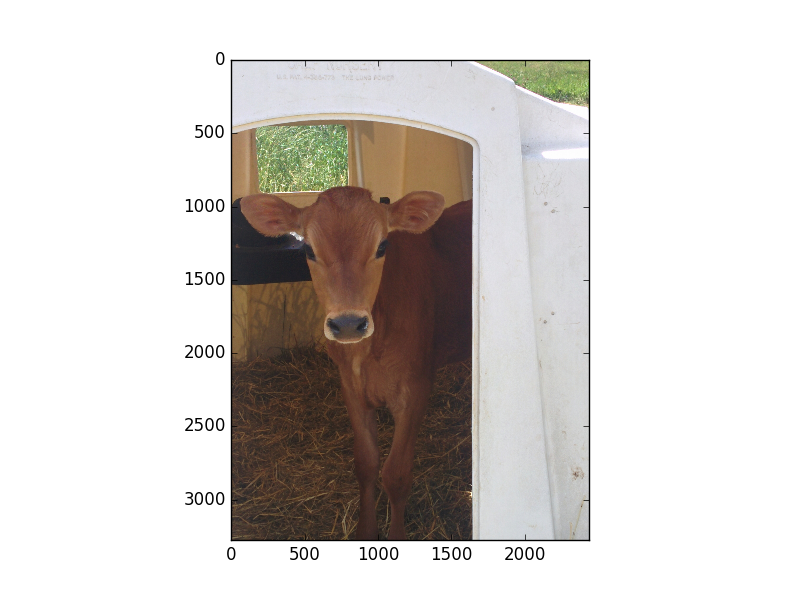
\includegraphics[width=2in]{calf_original} \\
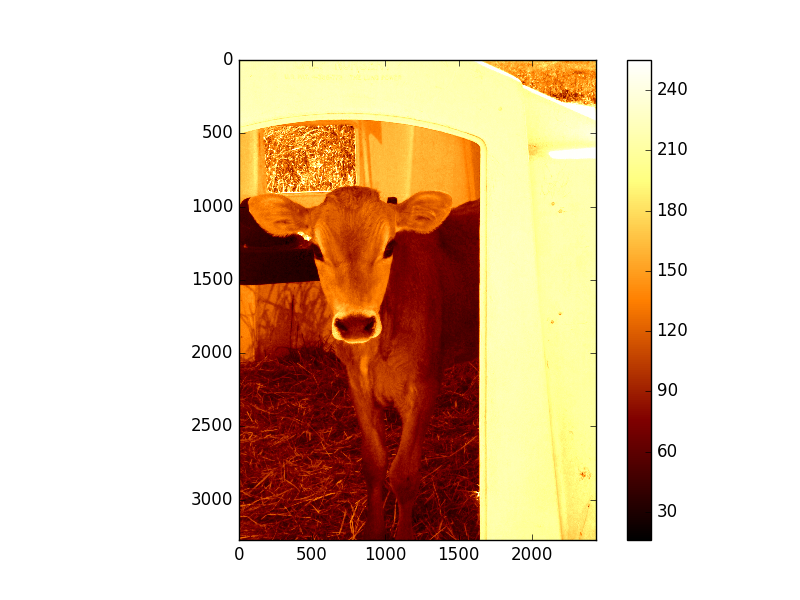
\includegraphics[width=2in]{calf_sequential} \\
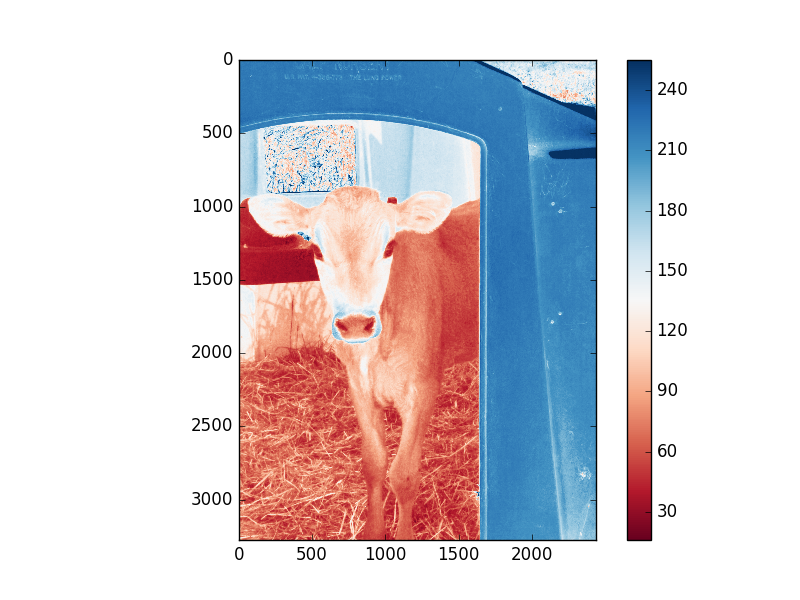
\includegraphics[width=2in]{calf_diverging} \\
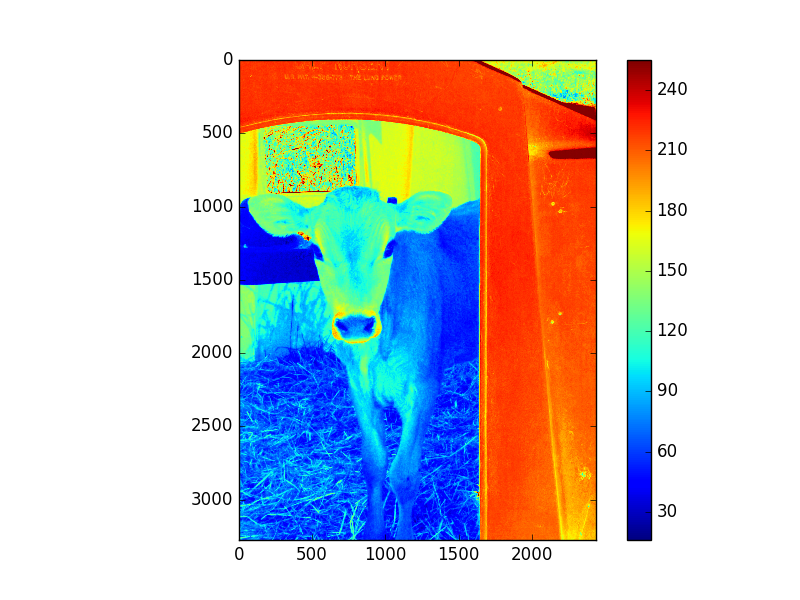
\includegraphics[width=2in]{calf_rainbow} \\
\caption{An image of a calf. The calf image plotted with a
sequential, diverging, and rainbow colormap. These images were created by the author.}
\end{figure}

Which color is bigger: red or blue? This illustrates the main problem
when designing a colormap: there is no natural ordering of the colors
from least to greatest. Some argue that there is a natural
ordering, namely by light wavelength. 
The brain's interpretation of this ordering produces the familiar rainbow spectrum of color hues
starting with red, then orange,
yellow, green, blue, and so forth \cite{colormapping}. This is the foundation for the rainbow colormap.
It was especially popular among physicists and soon grew to become the default
in many scientific software applications \cite{rainbowstill,matlab}. However,
this colormap was not created for data representation. It was designed based
on accurately representing light waves, not data.

Other colormaps take a different approach.
Color ordering can be constructed by choosing an appropriate color scheme.
There are three main types of color schemes that define a colormap.
Sequential color schemes vary in lightness but do not
vary in hue. If two sequential color schemes have different hues and are
connected at their lightest ends, it is called a diverging color scheme. Qualitative color
schemes vary in hues with little variation in lightness
and saturation \cite{colormapping}. The rainbow colormap uses a continuous,
qualitative color scheme. It is also known as a spectral scheme \cite{spectralschemes}
The images in Fig. 1
are examples of image data plotted with 
sequential, diverging, and rainbow colormaps.

What are the criteria for evaluating a colormap? Several authors have created
methods to evaluate color
choice. In one paper, color schemes are evaluated by
three variables of the CIELUV color model. The first
is color distance. Since CIELUV is a model of color distance, designed to
equally spaced colors on a colormap is considered good. The second variable is Linear separation.
This refers to “the ability to separate targets
from non-targets in the colour model being
used \cite{colorchoice}.” For example, suppose a doctor wants to identify
a tumor and uses a colormap to display the data. If the
colors are not linearly separable, it
will be more difficult to identify the tumor even if the
colors are mathematically different. The third variable
is color category, which refers to color regions where
there are both target and non-target elements \cite{colorchoice}.
 These characteristics do not account for multidimensional data projected into two-dimensional
space. CheckViz attempts to account for this problem
by using a perceptually uniform color coding so that
distortions such as those described above are accounted for when 
scientists want to visualize multidimensional data \cite{checkviz}.
The specific criteria of the color
model and color space must reflect the attributes of the colormap.

Colormaps have a variety of properties that make them unique and potentially
useful. However, there is controversy among scientists and visualization
experts over certain properties of the rainbow colormap. First, the rainbow
gradient is not a perceptually consistent ordering of colors. Similarly, it
is not perceptually uniform as the variation in lightness is inconsistent.
Finally, the rainbow colormap traverses through many
highly saturated colors in color space.

There are multiple advantages to using rainbow colormaps. For one,
it is clear that users tend to prefer it
over other colormaps for its aesthetic appeal
\cite{spectralschemes, choropleth, endofrainbow}. 
The variety in hue also can show relationships in the data better than
a sequential, single-hue colormap. The rainbow colormap also has a long
history of use in scientific publications and many are already used
to reading data from this colormap.

However, the advantages can also be disadvantages.
A human interpreter
might see signal where there is none. These false signals
are known as artifacts and they seem to occur more often
when the data lie in certain regions (as in
between blue, green, and yellow) \cite{colorchoice}.

\section{Color Perception}

One of the advantages of using perceptually uniform colormaps is
that they show the data accurately even if the colors do not appear
the same. Color perception can change for a number of reasons. When 
colors are placed near each other, it changes the way our eyes see that color.
The brain adjusts the amount of light that enters the eyes based
on external conditions. For example, colors appear more bright under diffused
light. Competing bright colors also diminishes the overall perception
of their brightness.

Some colormaps,
like Matlab's \textit{perula} colormap, are designed to be perceptually
uniform in the CIELAB color space \cite{viridis}. While not 
completely uniform, they provided the best notion of perceptual uniformity until
the CIECAM-02 models were developed in 2002.
The open source colormap \textit{viridis} created by Smith and van der Walt, uses
the CIECAM02-UCS color space to provide a perceptually uniform color space more
consistent with small differences in data values \cite{viridis}. There has been
little to no research on the effects of using this most recent model on colormap
development.

\begin{figure}
\centering
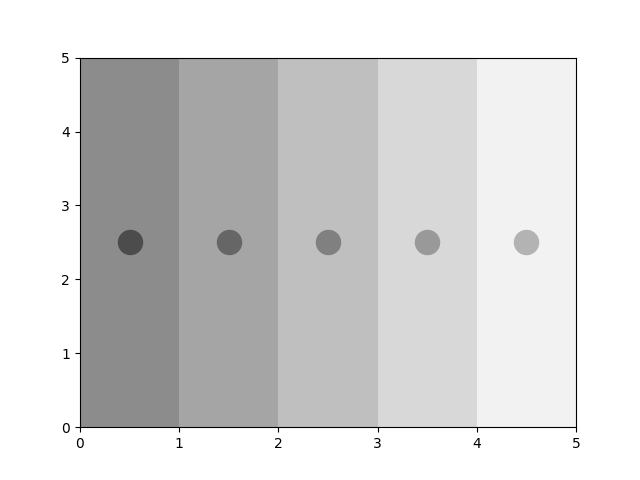
\includegraphics[width=2in]{tempcontrast} \\
\caption{An example of simultaneous contrast.}
\end{figure}

An example of color perception under different conditions is the 
color-of-the-dress meme that became popular in 2015. The picture was
sent on social media sites asking whether the dress was black and blue
or white and gold. This effect happens because our eyes perform a kind 
of normalization under different light conditions. This adjustment alters
the perception of what the colors look like \cite{viridis}.
The same shade of gray can appear very different as the surrounding color changes.
Even though the colors are the same, they appear to be 
different because of the context that they are in. This means that sometimes
we see color differences even when there are none.
Other times, color differences can't be detected easily or at all. This is 
especially common among people who have some form of color vision impairment,
or colorblindness.
Sometimes, when color encodings are converted to
grayscale, it can alter the perception of the data \cite{colorvblackwhite}.

In general, rainbow colormaps
are not perceptually uniform because the lightness is not consistent.
This has not stopped some from attempting to modify---and therefore preserve---the
rainbow colormap. The adjustments refer to the Munsell color specification system,
which describes color with hue, saturation, and lightness.
Sisneros et al created a colormap modification framework that smooths the variation
in luminance (or lightness) and chromaticity, which is a combination of saturation
and hue. Their method can be applied to any colormap to make it perceptually uniform.
However, they focused their efforts on improving the rainbow colormap, since it is still widely
used in science. Their improved rainbow colormap contains subdued colors that better
represent image data \cite{chasingrainbows}. 


\begin{figure}
\centering
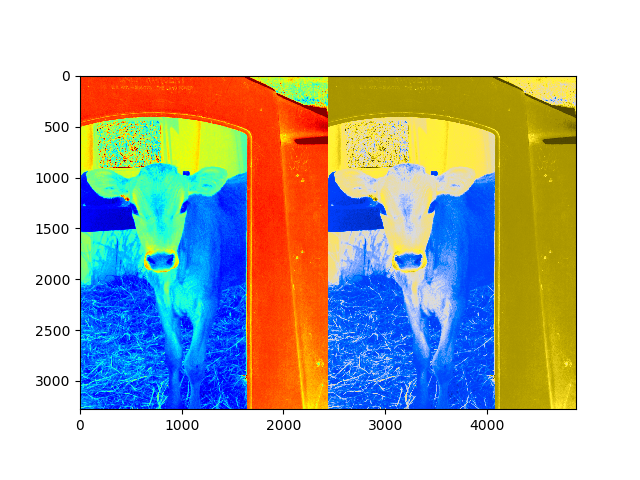
\includegraphics[width=2in]{colorblind_rainbow1.png}%
\caption{The rainbow colormaped image (left) and a colorblind approximation of the same image (right).}
\end{figure}

\subsection{Colorblindness}

Colorblindness results in colors falling on confusion lines---lines in which it
is difficult or impossible to distinguish between two colors \cite{colormapping}. People with full
color vision also have confusion lines and so in some sense are colorblind because 
we can't see the entire spectrum of light as colors. However, color deficient viewers
are special in that they do not see the normal range of colors as their peers.
There are multiple kinds of colorblindness.
Full color deficiency results in black and white vision and is very rare.
The most common form of color deficiency results in confusing shades of red and green \cite{colorchoice}.
%An example of a map colored with bright orange and green and what a deutoronome
%would see is given in Figure 3.

For these genetic color deficiencies, it seems reasonable to design data
visualizations with colorblindness in mind.
The estimated colorblind population is somewhere around 5-8\%
and affects mostly males of European descent \cite{colormapping}.
Unfortunately for the rainbow colormap,
the colors that a colorblind user sees are not the same as those seen by a person
with full color vision. Especially for high values, which are displayed in reds,
the variation in green is not easy to interpret for colorblind viewers \cite{mapcvi}. In fact,
though they are aesthetically pleasing, people are slower at interpreting data with
large variations in color and make more errors \cite{arteryvis}. Yet, colorblind people still seem
to get by fine.

Color deficient viewers use clues to distinguish between colors that easily confuse them.
Brewer has conducted extensive research into how color deficient
viewers interpret color-encoded information. She has suggested several ways in which 
maps and information visualizations can be designed to help color deficient viewers.
A common theme in her research, as well as others, is that colormaps are greatly
improved when the dark-to-light variation is controlled and used to show progression \cite{mapcvi}.
This is the idea behind perceptually uniform colormaps. Even when converted to black
and white, the visuals still preserve the nature of the data and are easy to interpret.

\section{Applications and Alternatives}

Readers of scientific literature will recognize the rainbow colormap. 
It appears often in scientific publications and has 
broad appeal in the scientific community
\cite{endofrainbow, rainbowstill, spectralschemes,choropleth}.
 Historically, rainbow colormaps like
MATLAB’s ‘jet’ have been the default colormaps used
in data-handling software \cite{matlab}. Despite its prevalence, 
many scientists oppose rainbow-gradient representations of data
\cite{rainbowstill, endofrainbow, viridis,arteryvis}.
 In one study, medical students were
asked to identify risk factors for heart disease in visualizations
of artery data. On average, the participants
using rainbow-colored visualizations took more time
and made more errors than participants using divergence-colored visualizations. 
Furthermore, the participants “thought they did well using the rainbow color
map even when in reality they did not perform as well
as the participants who used the diverging color map
\cite{arteryvis}.” This compelling evidence suggests
that the rainbow colormap is clearly inferior to other
colormaps.

Others disagree. They claim that users have learned to
read data with the rainbow colormap and prefer its
aesthetic appeal \cite{spectralschemes, choropleth}. One
experiment tested data interpretation accuracy under
diverging, sequential, and spectral (rainbow) color
schemes. “Of 63 subjects who evaluated spectral and
sequential schemes, 56 percent selected spectral as the
best...We had expected the spectral scheme to interfere
with map-reading accuracy and with understanding
map patterns, but this did not occur,” Brewer writes.
“Our subjects preferred the spectral scheme
and performed well with it \cite{spectralschemes}.”
 While the rainbow colormap did not outperform other colormaps, it
appears to do no harm. Users can accurately interpret
rainbow-colored data visualizations.

The controversy surrounding the rainbow colormap does not appear to be random.
Certain industries disagree on how much the rainbow colormap should be 
discouraged. There is general agreement that rainbow colormaps are not as 
precise as perceptually uniform colormaps in representing data 
\cite{colorvblackwhite}. However, this 
does not mean that rainbow colormaps are discouraged in all cases
 \cite{spectralschemes}. 
Among the many uses of the rainbow colormap in the
literature, the two most cited are
medical imaging and cartography. Both care deeply about the use of color in 
their respective fields \cite{colorguidelines, standardmedimg}. Even within
 these applications, the recommended use of the rainbow colormap differs
 depending on the context.
 
\subsection{Cartography}

Maps are used to show public health information, the spread of disease, weather
forecasts, and other demographic data. This information is important to
 public policy and public awareness. This information is almost always shown
 using color. Choosing an appropriate color scheme is not a trivial task. In her
article \textit{Mapping Mortality: Evaluating Color Schemes for Choropleth
Maps}, Cynthia Brewer shows that a judicious choice of color is ``worth 
the extra effort and expense'' because ``it permits greater accuracy in map
reading \cite{choropleth}.'' For public understanding of data, the rainbow colormap
seems to do no harm and users tend to prefer it.

Rainbows are not always good for maps, however. An assortment of colormaps were
developed and shown to be superior to rainbow schemes when used for oceaonography.
Sea level is an important metric in these contexts and a rainbow colormap poorly 
represents the coastline where land and sea meet. In this context, customized colormaps
outperform most other colormaps \cite{oceanography}. In contexts where the data are in a particular form
that the scientist knows, it is best to create a customized colormap that gives 
more accurate results.

\subsection{Medical Imaging}

The consequences for color misuse in medical imaging are more severe. Research
already shows that the potential for diagnostic errors increases when 
rainbow color schemes are used \cite{arteryvis}. In this research, color may not
be necessary and only used for convenience. However, some procedures require 
medical images that must be interpreted using color. In this case, it
is especially important that hardware components be standardized so that color
can be interpreted effectively. Since there are many manufacturers that produce
image processing software and display hardware, there is no consensus which 
color models or color mappings should be used by the medical community.
The Summit on Color in Medical Imaging
met to reach a consensus on how to standardize color use 
\cite{standardmedimg}. Images that are important to medicine but not exclusively
part of the community would not be held to these standards.

Bioinformatics and genetics are two fields related to medicine that 
could be exempt from the standards set in medical imaging. In fact, many tools
are being created now to analyze the vast amount of data that can be collected
in genetics. One such tool uses clustering techniques to find biomarkers in 
gene data. This software is written in Matlab and designed to run on Microsoft
Windows and Linux x86 \cite{marvis}. This specific choice of software uses an
older version of Matlab and uses the \textit{jet} default colormap. 
Software updates and hardware limitations make it difficult to change 
the visualization system. This may be another reason why doctors prefer
the rainbow visualization---it is just too difficult to change.

\subsection{Alternative Colormaps}

Many recognize that change is not easy. Some recommend changing 
colormap defaults instead of setting standards \cite{viridis}. That way, some 
consistency can be maintained while still allowing a little variation in the
implementation. This is the goal of visualization studies like the one 
carried out in the development of the HemoVis medical imaging program 
\cite{arteryvis}. This is especially important because it is not feasible for
every software to be written independently without dependencies on other
software.

\section{Conclusion}

Color is an essential attribute of data visualizations. Representing data
with color is best done through a colormap designed specifically for the data in
mind.
Colormaps require a vast amount of knowledge to be thoroughly constructed. It 
involves disciplines as different as engineering, computer science, graphic design,
and psychology. The recent development in color rendering technology has made it 
possible to develop and test many different colormaps. In particular, it seems clear
the rainbow colormap has many undesirable properties when trying to represent data.
It takes more time for viewers to interpret data with this colormap and they tend to
make mistakes when the data fall in areas where the color changes do not match 
equivalent changes in the data. There does not seem to be a problem in cartography
and people tend to prefer the rainbow colormap because it is familiar and aesthetically pleasing.
Despite these preferences, there is an increasing movement to replace the rainbow
colormap as the default colormap in scientific software \cite{matlab}. Recommended
alternatives are colormaps that are more perceptually uniform than the rainbow 
colormap. The variety of colors is diminished and the darkness-to-lightness progression
is more consistent with human perception of color change.

When data must be represented using color, most recommend using a perceptually
uniform colormap because it more accurately represents the data and is more 
friendly to colorblind or color impaired individuals. When colors cannot be changed
to accomodate for color impairment, redundancy can be added to the visualization
so as to encode the same information the color represents as a small icon or by using
a different visual variable such as position or size. In contexts where data
interpretation is to be precise and time-efficient, scientists are discouraged from
using the rainbow colormap. In applications where user preferences are valued over representational accuracy, the rainbow colormap is acceptable. However, scientists
are encouraged to use perceptually uniform colormaps to phase out the rainbow colormap
as a default and replace it with a colormap that more accurately represents a larger
variety of data.

We need more research in how to create custom colormaps. No good tools exists except for the things the viridis guys use, and that's only for perceptually uniform colormaps.


%\ifCLASSOPTIONcaptionsoff
%  \newpage
%\fi

\newpage

\bibliographystyle{ieeetr}
\bibliography{litreview}

\end{document}



